% !TEX root =  ../pers_schedules.tex

\section{Personalized Schedules for Patients in PRIAS}
\label{sec : pers_schedule_PRIAS}
To demonstrate how the personalized schedules work, we apply them to the patients enrolled in PRIAS. To this end, we divide the PRIAS dataset into a training dataset with 5264 patients and a demonstration dataset with three patients who never experienced GR. We fit a joint model to the training dataset and then use it to create personalized schedules for patients in demonstration dataset. We fit the joint model using the R package JMbayes \citep{rizopoulosJMbayes}, which uses the Bayesian methodology to estimate the model parameters.

\subsection{Fitting the Joint Model to PRIAS Dataset}
\label{subsec : jm_fit_prias}
The training dataset contains age at the time of induction in PRIAS, PSA levels and the time interval in which GR is detected, for 5264 prostate cancer patients. PSA was measured at every three months for first two years and every six months thereafter. To detect GR, biopsies were conducted as per the PRIAS schedule (Section \ref{sec : introduction}). For the longitudinal analysis of PSA we use $\log_2 \mbox{PSA}$ measurements instead of the raw data. This because the PSA scores take very large values around the time of disease progression, indicating that the underlying distribution for PSA is right skewed. The longitudinal sub-model of the joint model we fit is given by:
\begin{equation}
\label{eq : long_model_prias}
\begin{aligned}
\log_2 \mbox{PSA}(t) &= \beta_0 + \beta_1 (Age-70) + \beta_2 (Age-70)^2 + \sum_{k=1}^4 \beta_{k+2} B_k(t,\mathcal{K})\\ 
&+  b_{i0} + b_{i1} B_7(t, 0.1) + b_{i2} B_8(t, 0.1) +
\varepsilon_i(t).
\end{aligned}
\end{equation}
where $B_k(t, \mathcal{K})$ denotes the $k$-th basis function of a B-spline with three internal knots at $\mathcal{K} =\{0.1, 0.5, 4\}$ years, and boundary knots at zero and seven years. The spline for the random effects consists of one internal knot at 0.1 years and boundary knots at zero and seven years. The choice of knots was based on exploratory analysis as well as on model selection criteria AIC and BIC. Age of patients was median centered to avoid numerical instabilities during parameter estimation. For the relative risk sub-model the hazard function we fit is given by:
\begin{equation}
\label{eq : hazard_prias}
h_i(t) = h_0(t) \exp\big\{\gamma_1 (Age-70)  + \gamma_2 (Age-70)^2 + \alpha_1 m_i(t) + \alpha_2 m'_i(t)\big\}.
\end{equation}
where $\alpha_1$ and $\alpha_2$ are measures of strength of the association between hazard of GR and $\log_2 \mbox{PSA}$ value $m_i(t)$ and $\log_2 \mbox{PSA}$ velocity $m'_i(t)$, respectively. Since the PRIAS schedule depends only on the observed PSA values (via PSA-DT), the interval censoring observed in PRIAS is independent and non informative of the underlying health of the patient.

From the joint model fitted to the PRIAS dataset we found that only $\log_2 \mbox{PSA}$ velocity was strongly associated with hazard of GR. For any patient, a unit increase in $\log_2 \mbox{PSA}$ velocity led to an 11 times increase in the hazard of GR. The parameter estimates for the fitted joint model are presented in detail in Web Appendix C of the supplementary material. 

\subsection{Demonstration of Personalized Schedules}
\label{subsec : demo_prias_pers_schedule}
Using the demonstration dataset, we next present the functioning of personalized schedules based on expected time of GR and dynamic risk of GR. The first patient of interest is patient 3174. The evolution of PSA, repeat biopsy history and proposed times of biopsies for this patient are shown in the top panel of Figure \ref{fig : prias_demo_pid_3174}. It can be seen that the schedule of biopsy based on expected time of GR adjusts the times of biopsy according to the rise in hazard, which increases due steep rise in $\log_2 \mbox{PSA}$ velocity. More specifically, at year two the proposed biopsy time is 12.5 years whereas at year four it decreases to 5.3 years. On average, a biopsy scheduled using expected time of GR at year two should have a larger offset $O^S_j$ compared to the same at year four. This is because the standard deviation of $g(T^*_j)$, given by $\mbox{SD}_g(T^*_j) = \sqrt{\mbox{var}_g(T^*_j)}$, is considerably lower at year four as shown in the bottom panel of Figure \ref{fig : prias_demo_pid_3174}. In the figure it can be seen that the standard deviation also strongly depends on $\log_2 \mbox{PSA}$ velocity. As for the schedules based on dynamic risk of GR, the optimal $1 - \kappa$ value was found to be between 0 and 0.1 at all time points, because of the sharp rise in PSA values. This value of $\kappa$ corresponds to a time very close to the time of latest biopsy ($t=0$). Hence the biopsies are scheduled much earlier than those based on expected time of GR.

%Since no repeat biopsies were conducted for this patient in the time period we considered, $g(T^*_j)$ depends only on the PSA levels. 

\begin{figure}
\centerline{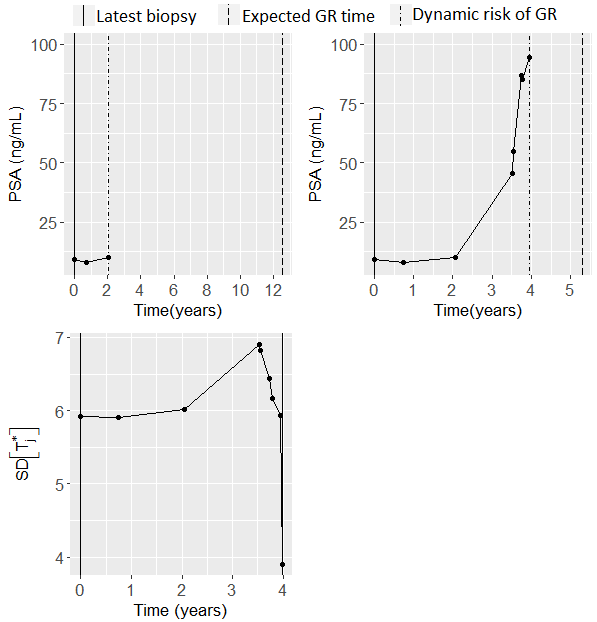
\includegraphics[width=\columnwidth]{images/prias_demo/case_3174.png}}
\caption{Top panel: Evolution of PSA, history of repeat biopsies and corresponding personalized schedules for patient 3174. Bottom Panel: History of repeat biopsies and $\mbox{SD}_g(T^*_j) = \sqrt{\mbox{var}_g(T^*_j)}$ over time for patient 3174.}
\label{fig : prias_demo_pid_3174}
\end{figure}

The demonstration of personalized schedules for the two other patients from the demonstration data set is discussed in Web Appendix D of the supplementary material.